\section{Introduction}\label{introduction}

\subsection{Introduction}\label{introduction-1}

\begin{frame}{Introduction - 自我介绍}

\begin{itemize}
\itemsep1pt\parskip0pt\parsep0pt
\item
  American pediatrician - 美国儿科医生
\item
  Lived in China for 22 years - 在中国生活22年
\item
  Married for 28 years (prettiest surgeon in Northwest China!) -
  结婚28年(中国西北最美的外科医生)
\item
  Two daughters (23 and 17 years old) - 有两个女儿(一个23岁,一个17岁)
\end{itemize}

\end{frame}

\begin{frame}{Family - 家庭}

\begin{figure}[htbp]
\centering
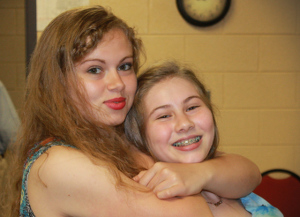
\includegraphics{./img/img_0002_300.jpg}
\caption{Lovely daughters!}
\end{figure}

\end{frame}

\subsection{Objectives}\label{objectives}

\begin{frame}{Objectives}

\begin{itemize}
\itemsep1pt\parskip0pt\parsep0pt
\item
  Participants will understand the importance of thinking about the
  kidney when facing disease states such as diabetes, HSP and spina
  bifida.
\item
  Participants will develop a plan for first steps evaluation and
  nephroprotection in the above mentioned disease states.
\end{itemize}

\end{frame}

\subsection{Abstract}\label{abstract}

\begin{frame}{Abstract}

The kidney is affected by a variety of disease states. Some are
intrinsically renal in origin but many are not. The generalist can be
expected to see patients with diabetes, HSP or spina bifida in the
course of a normal practice. All of these affect the kidney in different
ways. This talk will cover the primary reno-protective measures a
primary care physician can employ to make sure the patient's kidney will
last as long as possible in these disease states.

\end{frame}

\section{Diabetes}\label{diabetes}

\frame{\tableofcontents[hideothersubsections]}

\subsection{Diabetes in Children}\label{diabetes-in-children}

\begin{frame}{Diabetes in children}

\begin{itemize}
\itemsep1pt\parskip0pt\parsep0pt
\item
  Obesity is increasingly becoming a disease of younger and younger
  people.
\item
  IDDM is most commonly linked to renal disease
\item
  NIDDM is increasing in adolescents
\item
  Proteinuria on urinalysis
\item
  No edema on physical exam
\end{itemize}

\end{frame}

\subsection{Clinical findings}\label{clinical-findings}

\begin{frame}{Microalbuminuria}

\begin{itemize}
\itemsep1pt\parskip0pt\parsep0pt
\item
  Can occur in both insulin and non-insulin dependent diabetes
\item
  Not massive proteinuria

  \begin{itemize}
  \itemsep1pt\parskip0pt\parsep0pt
  \item
    protein:creatinine is low (usually total of 30-300mg albumin/g
    creatinine)
  \item
    albumin is normal
  \end{itemize}
\item
  Due to protein leak at the tubule, not at the glomerulus
\item
  Slow decline in GFR, leads to CKD over years
\item
  Most patients present after years of diabetic disease - 15+
\end{itemize}

\end{frame}

\begin{frame}{Hematuria}

\begin{itemize}
\itemsep1pt\parskip0pt\parsep0pt
\item
  Unusual
\item
  When present, think glomerular leak
\item
  Adults have ticks and fleas - Think about other causes of renal
  disease - IgA, membranous, etc.
\item
  Biopsy shows mesangial proliferation, glomerular sclerosis
\end{itemize}

\end{frame}

\subsection{Renal protection}\label{renal-protection}

\begin{frame}{Renal protection}

\begin{itemize}
\itemsep1pt\parskip0pt\parsep0pt
\item
  Consider ACEI to protect the tubules
\item
  Monitor blood pressure and treat accordingly
\item
  Control diabetes to slow progression of renal disease

  \begin{itemize}
  \itemsep1pt\parskip0pt\parsep0pt
  \item
    Weight reduction
  \item
    Lipid control (rarely needed in peds)
  \end{itemize}
\item
  No protein restriction (in peds)
\end{itemize}

\end{frame}

\begin{frame}{Monitoring}

\begin{itemize}
\itemsep1pt\parskip0pt\parsep0pt
\item
  Yearly screens for proteinuria in all diabetics
\item
  q3 Month check of protein:creatinine ratio for patients with
  demonstrated proteinuria

  \begin{itemize}
  \itemsep1pt\parskip0pt\parsep0pt
  \item
    Goal is less than 1000mg/day protein excretion (less than 500 is
    even better!)
  \end{itemize}
\item
  Blood pressure monitoring
\item
  Follow potassium in patients on ACEI or ARB
\end{itemize}

\end{frame}

\section{Questions?}\label{questions}

\begin{frame}{Questions? 提问题?}

\begin{figure}[htbp]
\centering
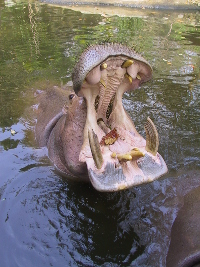
\includegraphics{./img/img_0510_200.jpg}
\caption{}
\end{figure}

\end{frame}
